\documentclass{article}
\usepackage[utf8]{inputenc}
\usepackage[tmargin=2in]{geometry}
\usepackage{setspace}
\usepackage{verbatim}
\usepackage{listings}
\usepackage{amsmath}
\usepackage{amsthm}
\usepackage{amssymb}
\usepackage{pgfplots}
\usepackage{graphics}
\usepackage{graphicx}
\usepackage{color}
\usepackage{float}

\definecolor{DarkGrey}{rgb}{0.1,0.1,0.1}
\lstdefinestyle{bash}
{ language=Bash,
	backgroundcolor=\color{white},
	keywordstyle=\color{BlueViolet}\bfseries,
	commentstyle=\color{Grey},
	stringstyle=\color{Red},
	showstringspaces=false,
	basicstyle=\footnotesize\color{black},
	numbers=none,
	captionpos=b,
	tabsize=4,
	breaklines=true
}

\definecolor{mygreen}{rgb}{0,0.6,0}
\definecolor{mygray}{rgb}{0.5,0.5,0.5}
\definecolor{mymauve}{rgb}{0.58,0,0.82}

\lstset{
	backgroundcolor=\color{white},   % choose the background color
	basicstyle=\footnotesize,        % size of fonts used for the code
	breaklines=true,                 % automatic line breaking only at whitespace
	captionpos=b,                    % sets the caption-position to bottom
	commentstyle=\color{mygreen},    % comment style
	escapeinside={\%*}{*)},          % if you want to add LaTeX within your code
	keywordstyle=\color{blue},       % keyword style
	stringstyle=\color{mymauve},     % string literal style
}


\doublespacing
\pagenumbering{gobble}

\renewcommand{\qedsymbol}{$\blacksquare$}
\graphicspath{ {./} }

\begin{document}

\begin{center}
Dustin McAfee (dmcaffe2) \& Alan Grant (agrant16)\\
COSC 560 \\
Programming Assignment 1 \\
Spring 2018 \\
\end{center}

\section*{How to Set Up and Run Python Server}
\begin{center}
	Unzip zipfile, "cs560\_server.zip", and use the following commands: \\
	\begin{lstlisting}[language=bash, style=bash]
		$ chmod u+x cs560_server.py 
		$ chmod u+x cgi-bin/formsubmit.cgi
		$ chmod u+x cgi-bin/mathcgi.cgi
	\end{lstlisting}
	The python server runs on http://localhost:8080 by default, but takes a port number as an argument if the user wishes to use a different port. To run the server call \\
	\begin{lstlisting}[language=bash, style=bash]
		$ ./cs560_server.py [port_number]
	\end{lstlisting}
	If starting on the default port 8080, the output should be \\
	\begin{lstlisting}[language=bash, style=bash]
		Starting server on 8080...
		Port acquired. Listening...
		Press CTRL+C to shutdown server.
	\end{lstlisting}
\end{center}
The server is now up and running, and can be accessed by typing in the server machine's IP address into another machine and connecting to the correct port. In this write-up, we will continue to use localhost as seen in the screenshots. \\
The server machine prints to standard out when there is an http request. A screenshot is shown below in Figure \ref{fig:req}: \\
\begin{figure}[H]
	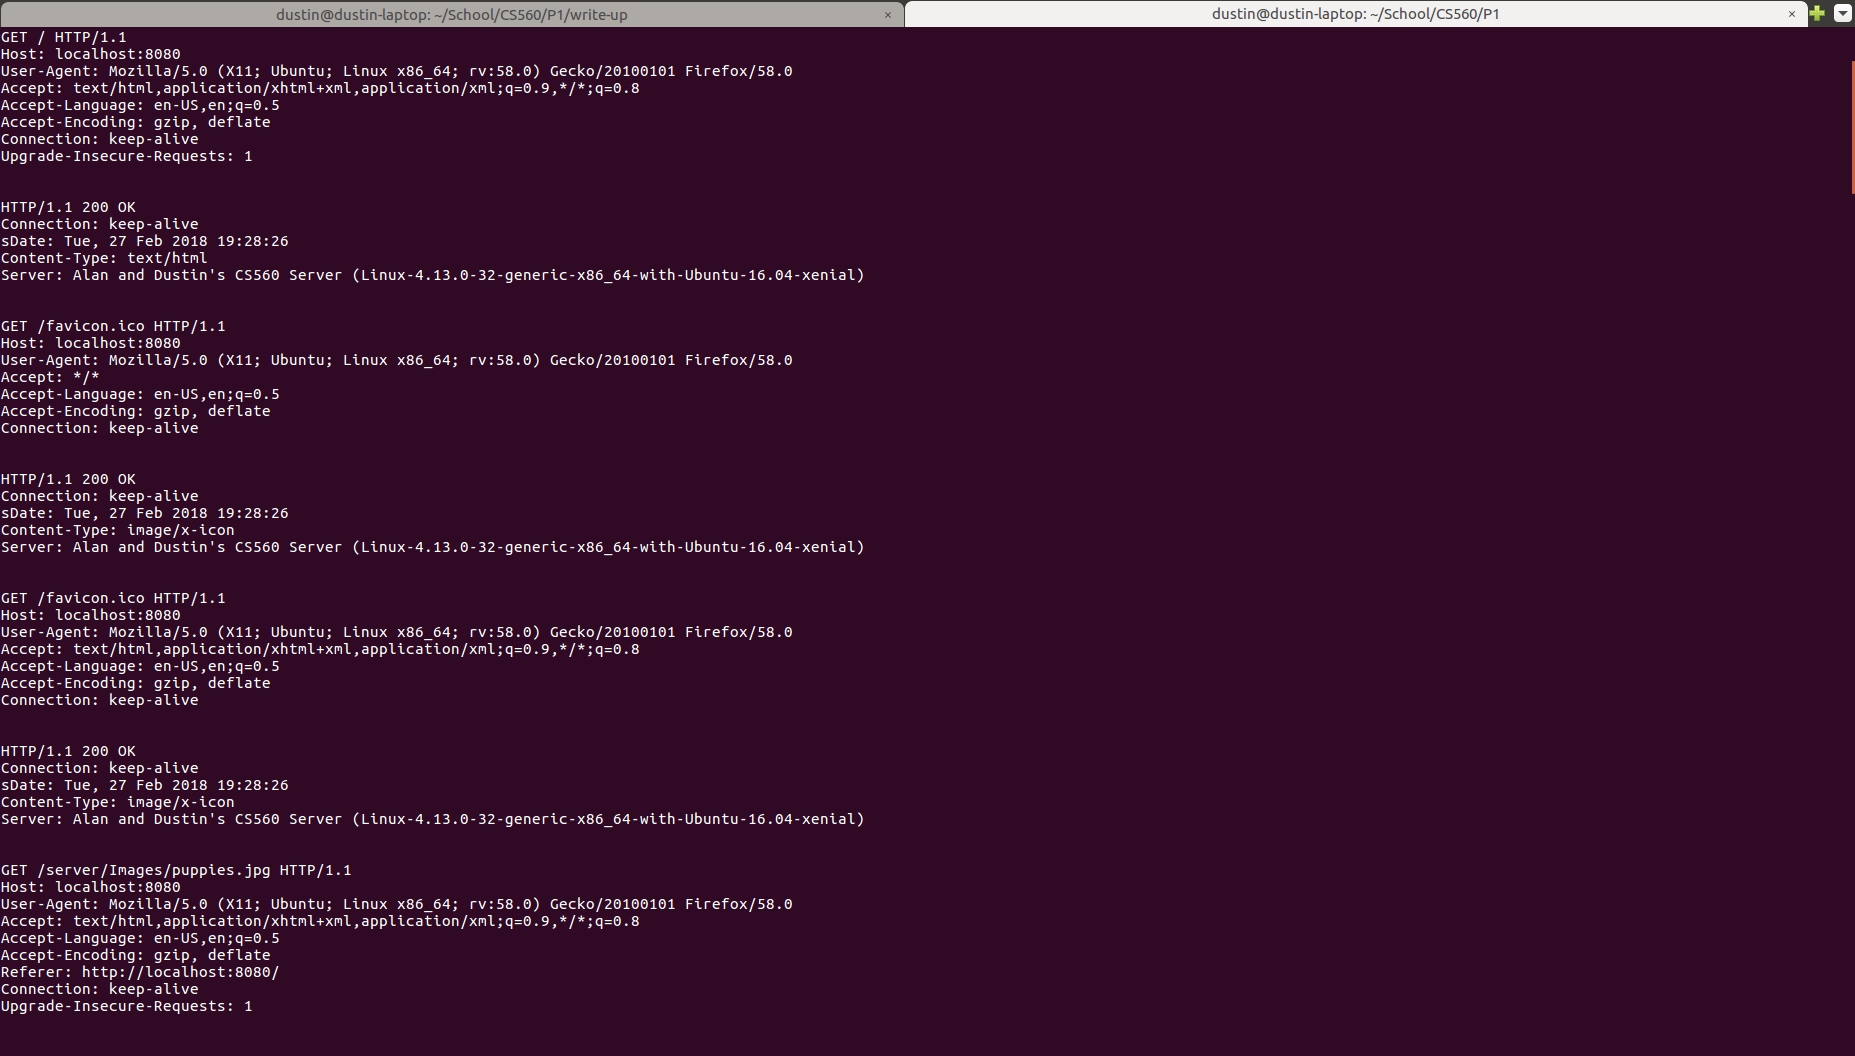
\includegraphics[width=\textwidth]{HttpResponse.png}
	\centering
	\caption{Output of HTTP requests}
	\label{fig:req}
\end{figure}
To end the server, press Control+C. When connected to the server via a browser (firefox or chrome), the index.html page will show (Figure \ref{fig:index} below). On this page, the user can view the files on the server, write to a file on the server via the form submit of a name and message, or use a CGI script to operate on two numbers.
\begin{figure}[H]
	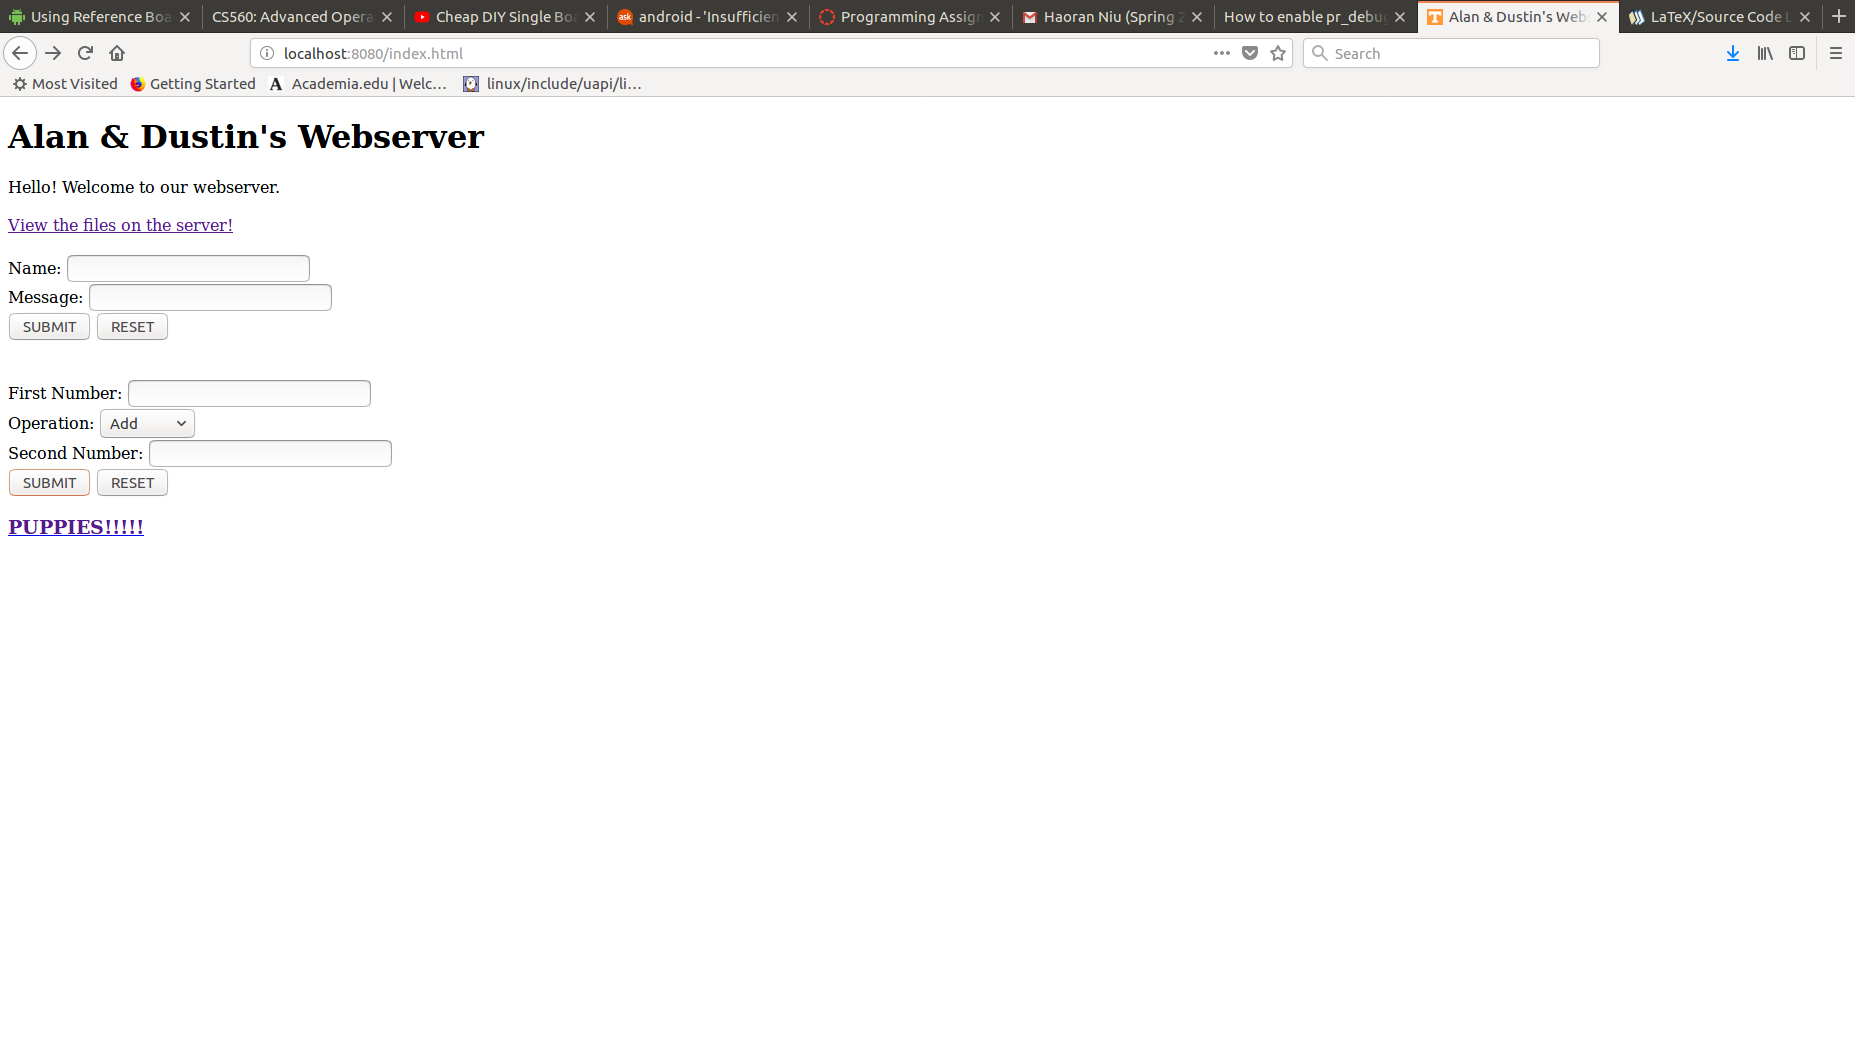
\includegraphics[width=\textwidth]{index.png}
	\centering
	\caption{index.html}
	\label{fig:index}
\end{figure}
The execution of the server code happens as follows: \\

After the CS560Server initializes, the serve\_forever member function (lines 379 to 391) starts an infinite loop to await connections. When a connection from a new client is established it creates a new thread for that client and starts the \_threaded\_response member function (lines 350 to 376). This is discussed further in Section 1. The \_threaded\_response function loops forever waiting for new requests from the client it is serving. If no new requests are received, or the client times out, the connection is closed. When a request is received from the client an instance of the CS560Handler class is created to parse the request and build the appropriate response. The requests is passed to the  CS560Handler member function handle (lines 54 to 88) which starts the parsing and response procedure using the \_do\_GET (lines 138 to 187, responsible for responding to GET requests) and \_gen\_headers (lines 190 to 234, responsible for generating response headers) member functions (coveredin Section 2). The handler will then decide which action is appropriate and call the correct member function:  server the request file for static file transfers (part of the \_do\_GET member function), \_run\_script (lines 237 to 260, responsible for running CGI scripts on the server: covered in Section 5, and for form submission: covered in Section 6), list\_dir (lines 263 to 297, responsible for listing directory contents: covered in section 3). The call to run\_script will invoke a script from the cgi-bin directory: mathcgi.cgi (covered in Section 5) or formsubmit.cgi (covered in Section 6). 

\section*{1: Single and Multiple Connection}

If only one client is connected the server runs in serial mode where only a single thread is parsing requests and responding. When a new client connects a the server\_forever (Listing \ref{code:serve_forever}) function spawns a new thread running the \_threaded\_response function (Listing \ref{code:_threaded_response}). For this process we used Python's \_thread module. The code for these sections is below. 

	\lstinputlisting[firstline=375,lastline=387,language=python,caption=CS560Server.serve\_forever,label=code:serve_forever]{../cs560_server.py}

\
	\lstinputlisting[firstline=346,lastline=372,language=python,caption=CS560Server.\_threaded\_response,label=code:_threaded_response]{../cs560_server.py}

\
\section*{2: HTTP GET Requests with Query and Header Parsing}

When a request is recieved from a client the thread associated with the client creates an instance of CS560Handler and uses that instance to parse the request and respond. CS560Handler.handle (Listing \ref{code:handle}) parses the request to find the method and the requested content. 

	\lstinputlisting[firstline=53,lastline=85,language=python,caption=CS560Handler.
	handle,label=code:handle]{../cs560_server.py}
	
Once the method and content are parsed CS560Handler.\_respond (Listing \ref{code:_respond}) is called. This function assesses the request method and decides on appropriate action. If the request is a GET or a HEAD it calls \_do\_GET to perform the proper action. If it is any other request method a basic html page to display the error is generated and the server responds with a 405 error (unsupported request method).
 
	\lstinputlisting[firstline=97,lastline=132,language=python,caption=CS560Handler.\_respond,label=code:_respond]{../cs560_server.py}
	

If the method is accepted CS560Handler.\_do\_GET (Listing \ref{code:_do_GET} below) is called. This function reacts appropriately. If the requested content is a static file it is converted to a bytes stream and prepared for sending. If the requested content is a directory it will call CS560Handler.\_list\_dir (more in Section 3). If the requested content containsa query string it will parse it. Query parsing is for running CGI scripts, such as form submission. If the CS560Handler.\_do\_GET member function finds a query that needs to be parsed, it invokes the CS560Handler.\_run\_script member function. More about this in Sections 5 and 6. \\

	\lstinputlisting[firstline=135,lastline=184,language=python,caption=CS560Handler.\_do\_GET,label=code:_do_GET]{../cs560_server.py}


	An example of an HTTP GET request would be the initial access to the index.html file as shown in Figure \ref{fig:index}. The output from the server of multiple HTTP requests is shown in Figure \ref{fig:req}. The output of the initial HTTP GET requests of the index.html page and its icon is shown below.
	
	\begin{lstlisting}[language=bash, style=bash]
	GET /index.html HTTP/1.1
	Host: localhost:8080
	User-Agent: Mozilla/5.0 (X11; Ubuntu; Linux x86_64; rv:58.0) Gecko/20100101 Firefox/58.0
	Accept: text/html,application/xhtml+xml,application/xml;q=0.9,*/*;q=0.8
	Accept-Language: en-US,en;q=0.5
	Accept-Encoding: gzip, deflate
	Connection: keep-alive
	Upgrade-Insecure-Requests: 1


	HTTP/1.1 200 OK
	Connection: keep-alive
	sDate: Tue, 27 Feb 2018 21:10:02
	Content-Type: text/html
	Server: Alan and Dustin's CS560 Server (Linux-4.13.0-32-generic-x86_64-with-Ubuntu-16.04-xenial)


	GET /favicon.ico HTTP/1.1
	Host: localhost:808
	User-Agent: Mozilla/5.0 (X11; Ubuntu; Linux x86_64; rv:58.0) Gecko/20100101 Firefox/58.0
	Accept: text/html,application/xhtml+xml,application/xml;q=0.9,*/*;q=0.8
	Accept-Language: en-US,en;q=0.5
	Accept-Encoding: gzip, deflate
	Connection: keep-alive


	HTTP/1.1 200 OK
	Connection: keep-alive
	sDate: Tue, 27 Feb 2018 21:10:02
	Content-Type: image/x-icon
	Server: Alan and Dustin's CS560 Server (Linux-4.13.0-32-generic-x86_64-with-Ubuntu-16.04-xenial)
	\end{lstlisting}

\section*{3: Automatic Directory Listing}
	If the HTTP request is a directory, then \_do\_GET will call CS560Handler.\_list\_dir (Listing \ref{code:_list_dir} below). This dynamically generates a link page of the contents of the directory (Figure \ref{fig:dir_list}). A link to the directory titled "View files on the server!" is on the index page as shown in Figure \ref{fig:index}. This link lists the files in the server directory.
	
	\lstinputlisting[firstline=260,lastline=294,language=python,caption=CS560Handler.\_list\_dir,label=code:_list_dir]{../cs560_server.py}
	
	\begin{figure}[H]
		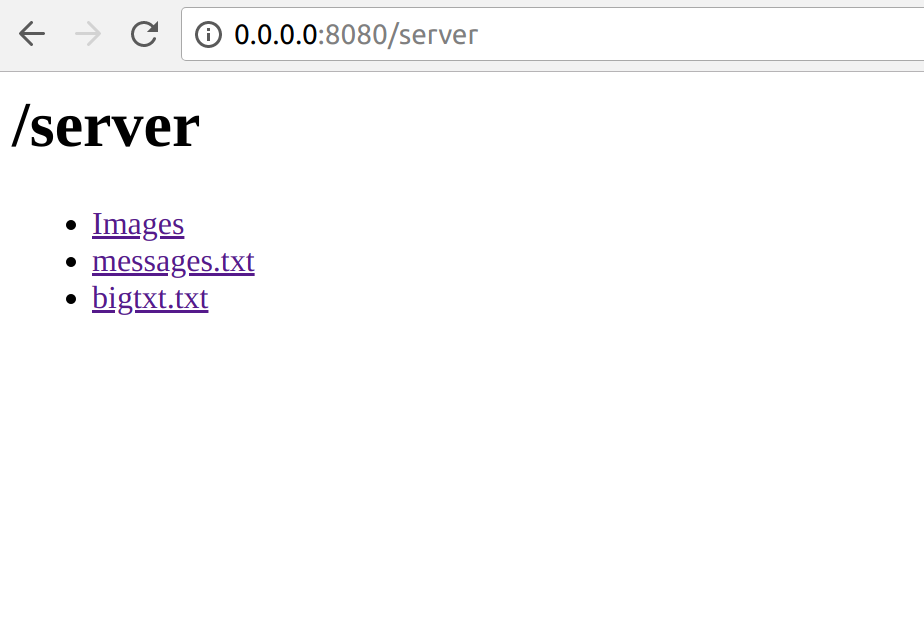
\includegraphics[scale=0.3]{dir_list.png}
		\centering
		\caption{Static File Transport}
		\label{fig:dir_list}
	\end{figure}
	
\section*{4: Static File Transport}
	The CS560Handler.\_do\_GET member function (from Listing \ref{code:_do_GET}) checks to see if the request is a supported file with the pathlib library call to is\_file(). If it is, then it reads and returns the contents of the file. An example of this kind of request is shown in Figure \ref{fig:doggo} below where a .jpg file was requested.

	\begin{figure}[H]
		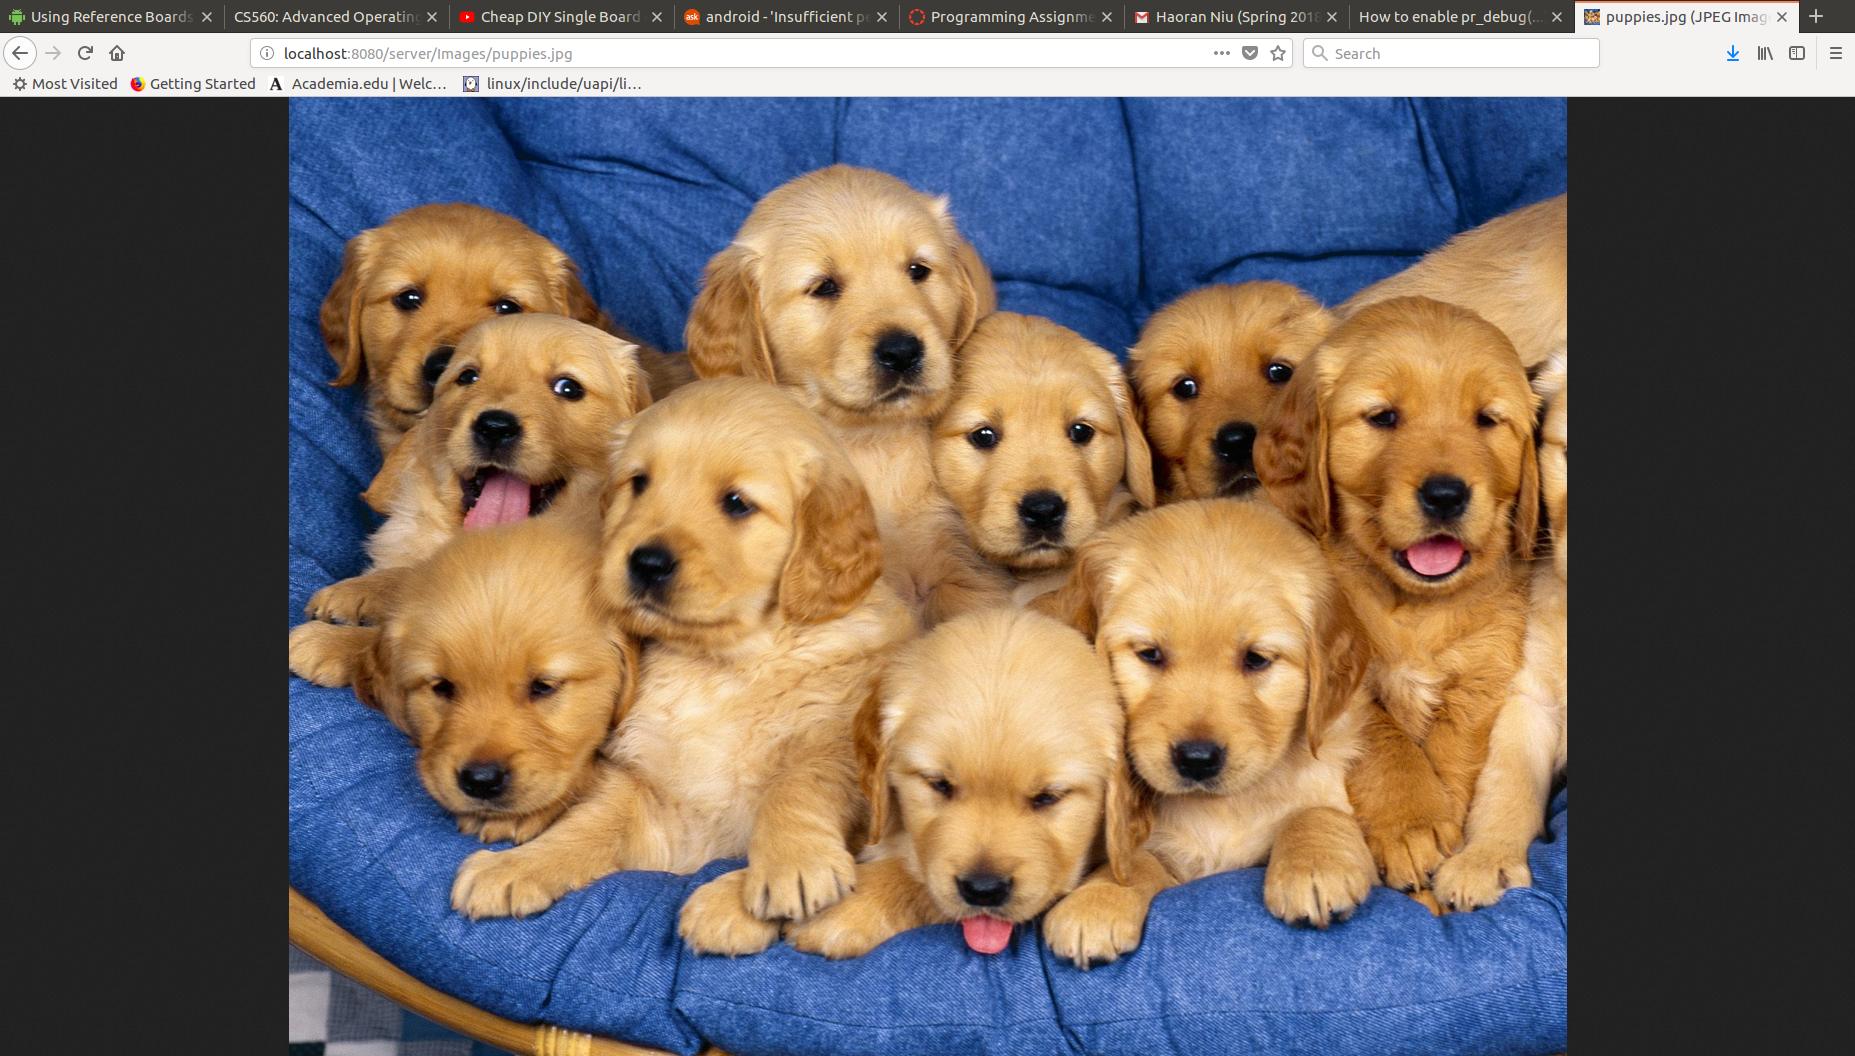
\includegraphics[width=\textwidth]{doggo.png}
		\centering
		\caption{Static File Transport}
		\label{fig:doggo}
	\end{figure}

	This can be done from the index page (Figure \ref{fig:index}) from the link titled "PUPPIES!!!!!", or from viewing the directory listing and downloading files from the server.
	
\section*{5: Basic CGI support}
	The CS560Handler.\_do\_GET member function (Listing \ref{code:_do_GET}) determines whether the request contains a query string. If so, then a CGI script is to be ran on the server using a GET request, by invoking the member function CS560Handler.\_run\_script (shown in Listing \ref{code:_run_script} below) which parses the arguments from the CGI script, and invokes the script.

	\lstinputlisting[firstline=234,lastline=257,language=python,caption=CS560Handler.\_run\_script,label=code:_run_script]{../cs560_server.py}
	
	The index page (Figure \ref{fig:index}) contains fields for two numbers and a submit button that invokes the cgi-bin/mathcgi.cgi script with the two numbers and an operation as arguments. It then generates a page with the result. This result page is shown in Figure \ref{fig:mathresult} below.

	\begin{figure}[H]
		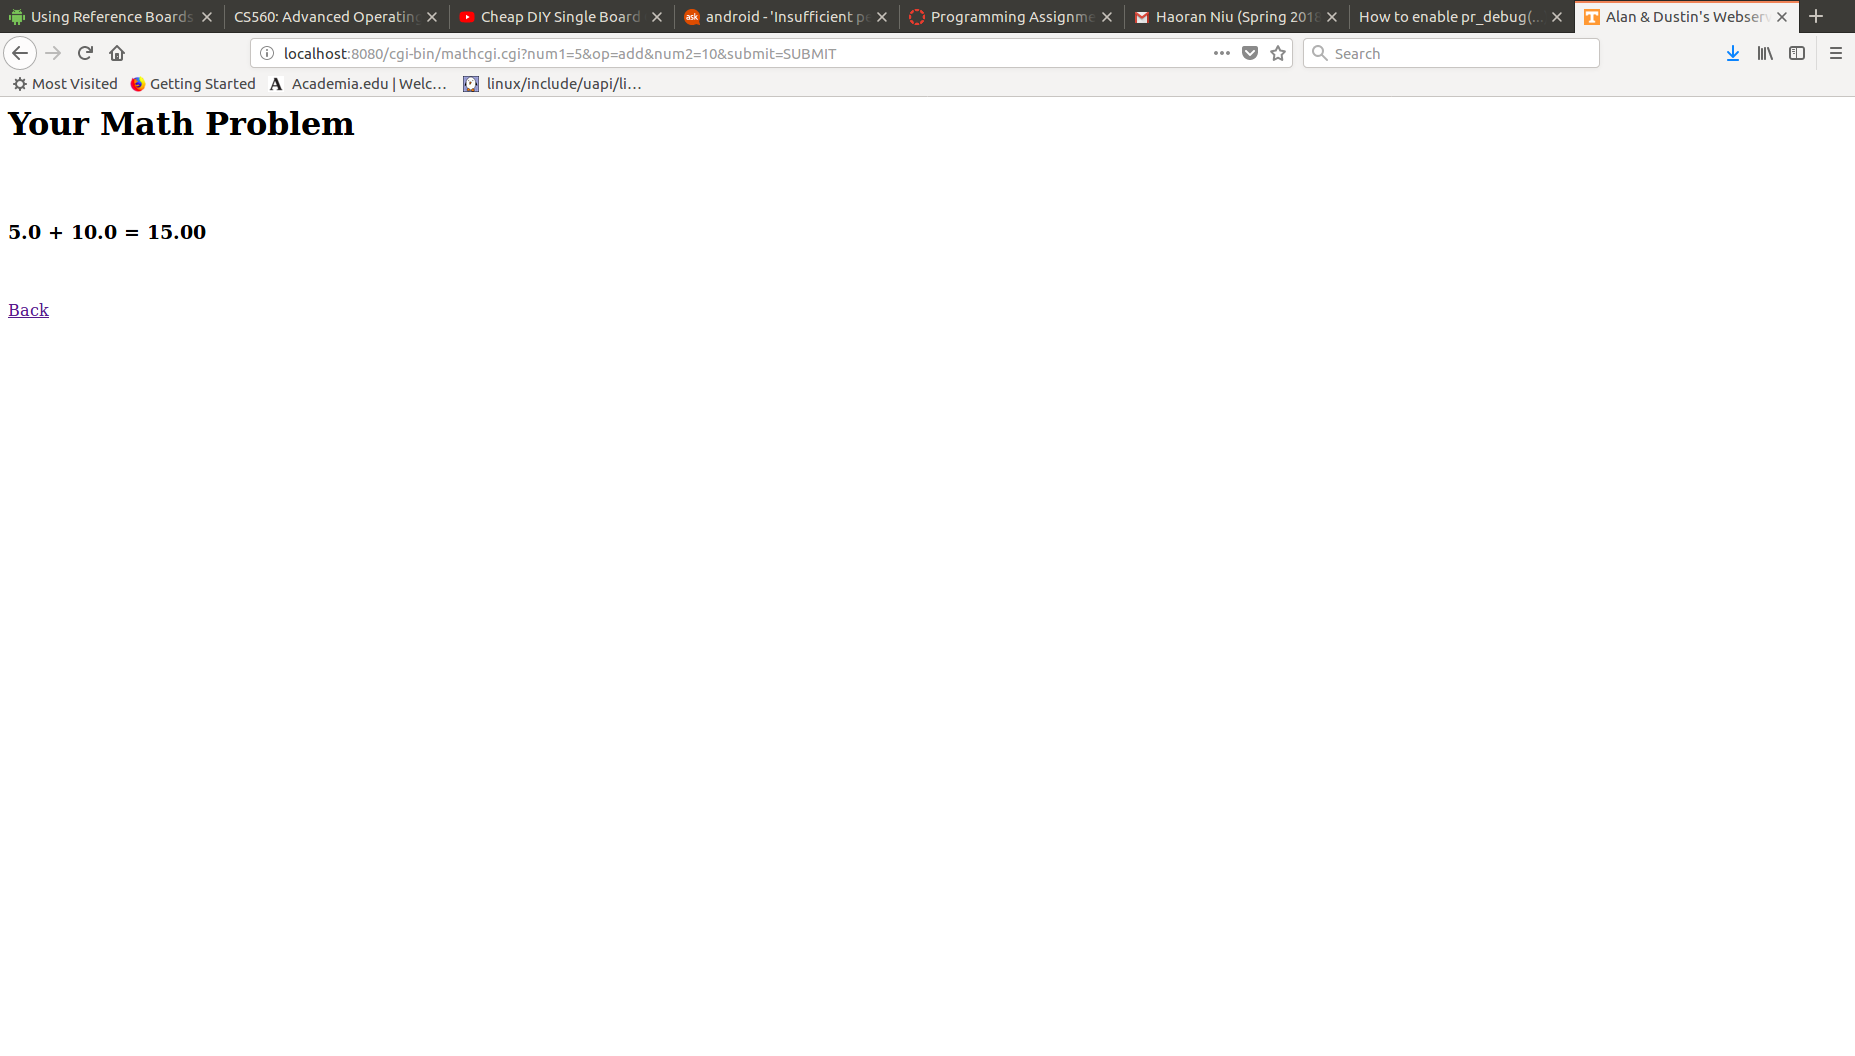
\includegraphics[width=\textwidth]{math.png}
		\centering
		\caption{Result of CGI script}
		\label{fig:mathresult}
	\end{figure}

\section*{6: Form Submit to File}
	The CS560Handler.\_run\_script (Listing \ref{code:_run_script}) is responsible for invoking CGI scripts. The cgi-bin/formsubmit.cgi (Listing \ref{code:formsubmit} below) script reads the "Name" and "Message" fields on the index page (Figure \ref{fig:index}) and appends them to the server/messages.txt file. After submission, the script generates a "Message Submitted" message that is displayed to the browser, along with a back button that links to the index page. 

	\lstinputlisting[language=python,caption=formsubmit.cgi,label=code:formsubmit]{../cgi-bin/formsubmit.cgi}

	To view these messages visit or download localhost:8080/server/messages.txt. An example file is shown in Figure \ref{fig:messages} below.

	\begin{figure}[H]
		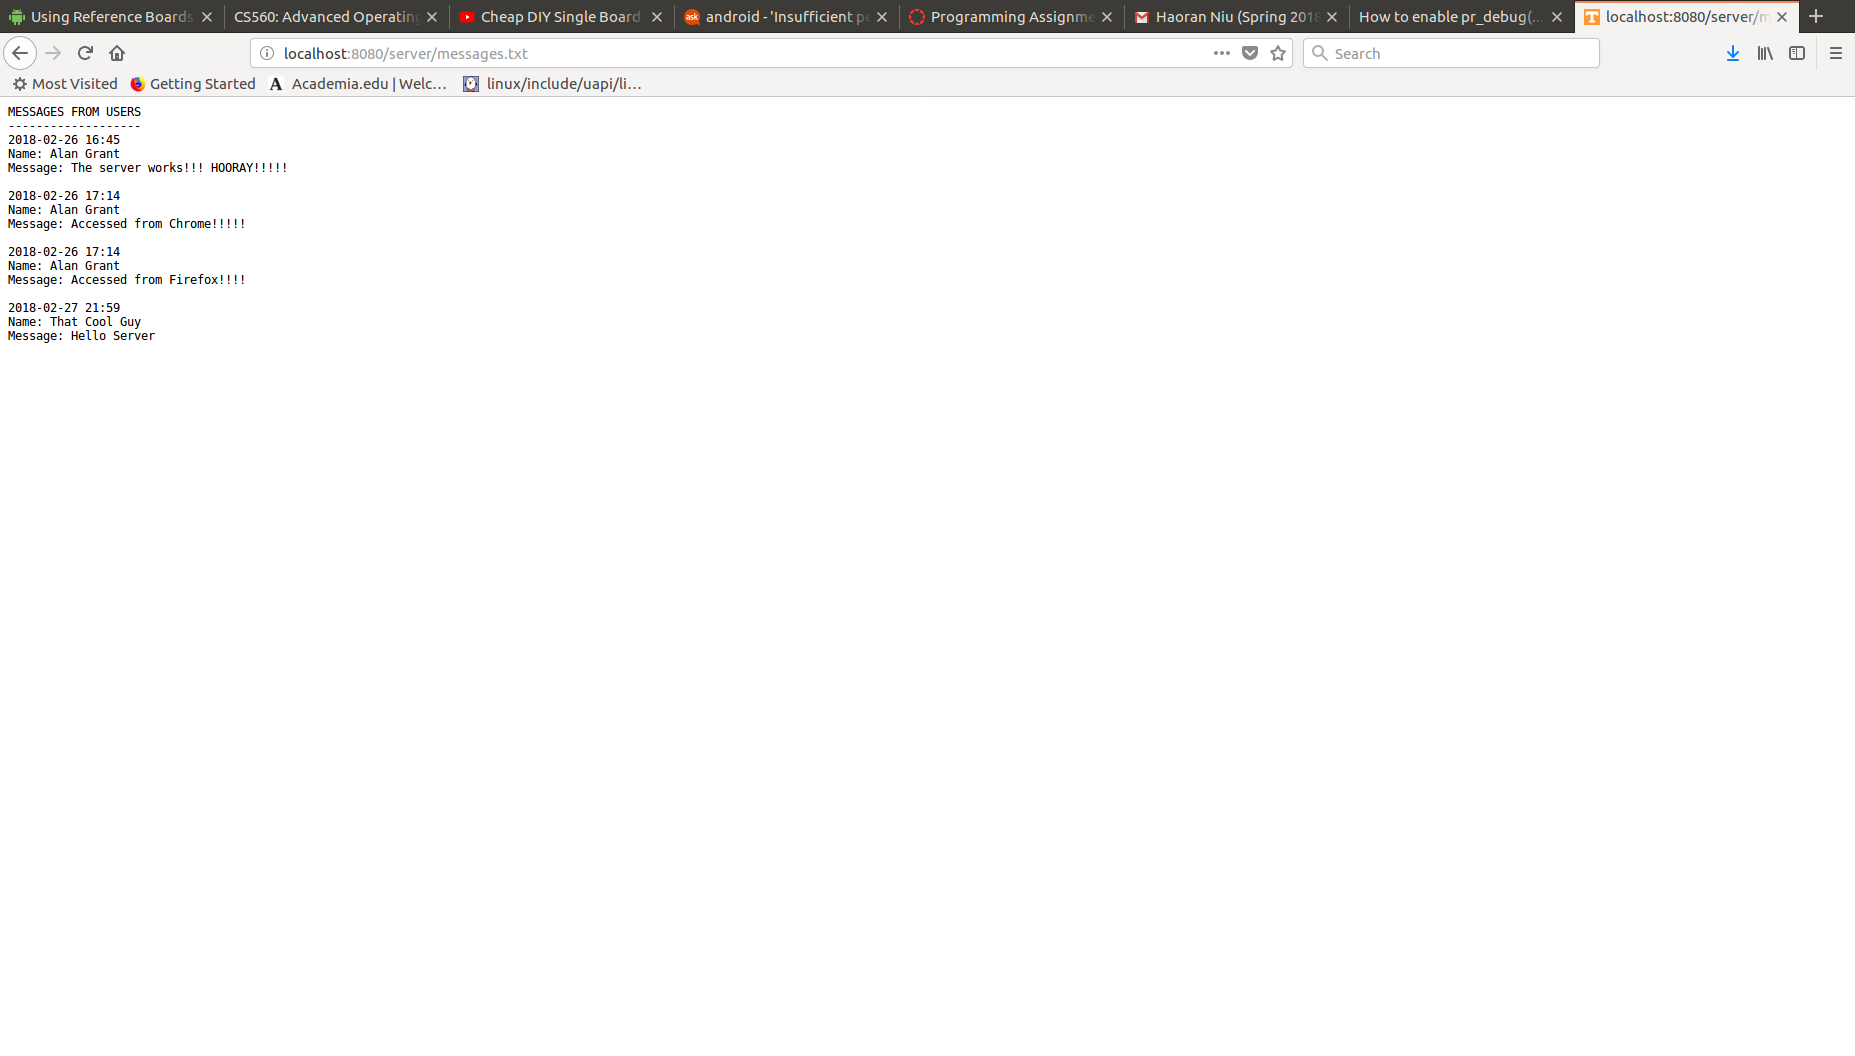
\includegraphics[width=\textwidth]{messages.png}
		\centering
		\caption{Example messages.txt File}
		\label{fig:messages}
	\end{figure}

\end{document}

